Die Korrekturen die auf das rohe Spektrum angewandt werden basieren auf der Monte Carlo Simulationen, aus der auch die Templates für diese Analyse stammen.
\newline
Die Detektorakzeptanz spiegelt dabei die Abdeckung des EMCals wider.
Sie berechnet sich aus dem Verhältnis der \textit{Clusterpaare}, die auf das EMCal treffen, zu den produzierten \textit{Clusterpaaren}.
\newline
Die Effizienz berechnet sich aus der Division der \textit{Clusterpaare} aus dem Template des Signals geteilt durch die Anzahl der akzeptierten \textit{Clusterpaaren}.
Für die Effizienz wird der $m_\text{inv}$ Bereich zum Zählen benutzt, der auch für die Bestimmung des rohen Spektrums benutzt wurde.
\begin{figure}[t!]
\centering
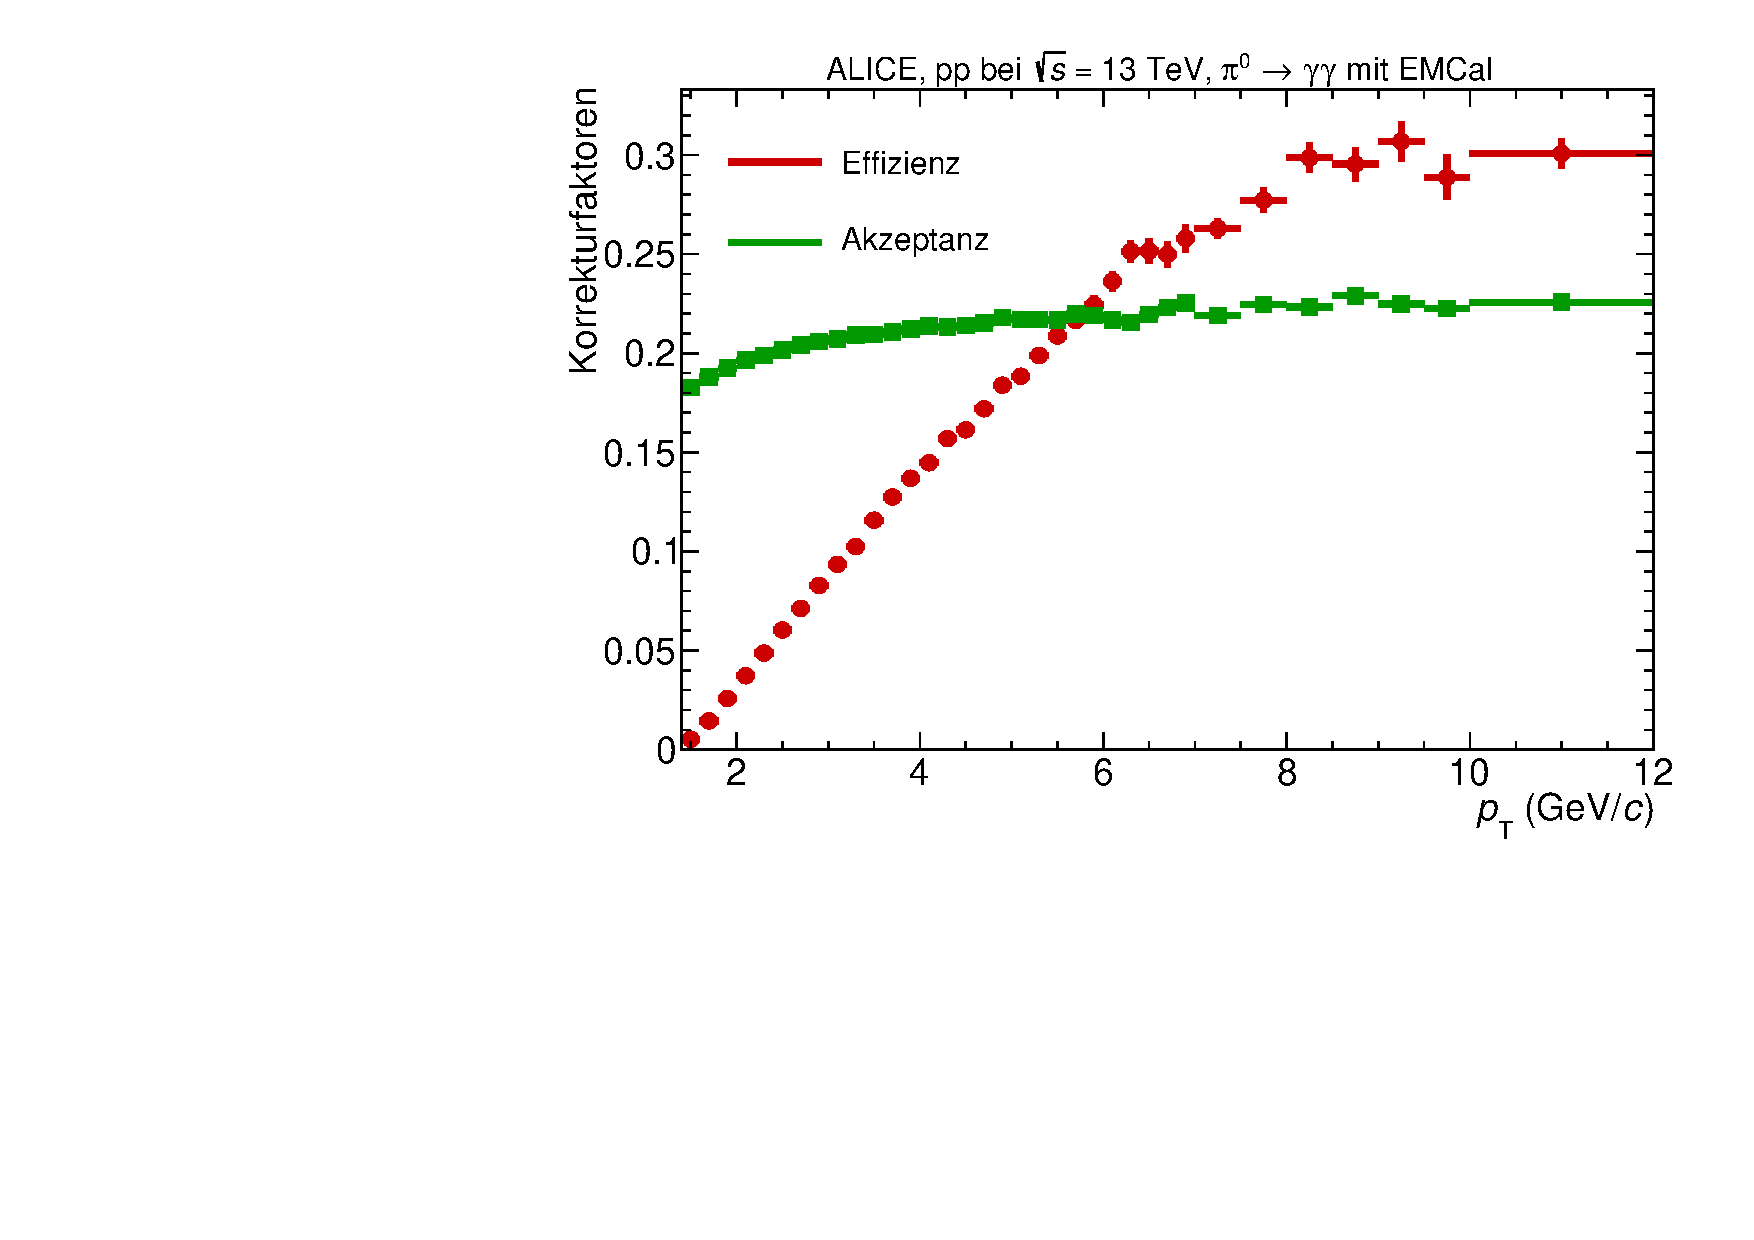
\includegraphics[width=.65\linewidth]{Korrekturfaktoren_Data_2016.pdf}
\caption{Detektorakzeptanz und Effizienz in Abhängigkeit von $p_\text{T}$.
}
\label{fig:Korrekturen}
\end{figure}
\newline
Durch das Korrigieren des rohen Spektrums mit der Detektorakzeptanz und der Effizienz, wird die Anzahl der detektierten und extrahierten $\pi^{0}$ auf die Anzahl der produzierten $\pi^{0}$ korrigiert.
Abbildung \ref{fig:Korrekturen} zeigt die beiden Korrekturgrößen Detektorakzeptanz und Effizienz.
\newline
Zerfällt ein $\pi^{0}$ in zwei Photonen, so fliegen die Photonen im System des $\pi^{0}$ entgegengesetzt zu einander weg, $\theta_{\gamma\gamma}$ beträgt in diesem System $180^{\circ}$.
Abhängig vom $p_\text{T}$ den ein $\pi^{0}$ im Laborsystem hat verringert sich $\theta_{\gamma\gamma}$.
Je größer $p_\text{T}$ umso kleiner $\theta_{\gamma\gamma}$.
Deshalb treffen beide Photonen aus einem $\pi^{0}$-Zerfall bei niedrigem $p_\text{T}$ seltener auf das EMCal.
Aus diesem Grund steigt die Detektorakzeptanz leicht an.
\newline
Durch die Anforderungen an die \textit{Cluster} werden unter anderem auch \textit{Cluster} ausgeschlossen, deren zugrunde liegende Teilchen aus dem Zerfall eines $\pi^{0}$ stammen, aber zu wenig Energie besitzen.
Gerade asymmetrische Zerfälle, bei denen der Anteil der zur Verfügung stehenden Energie ungleichmäßig auf die Zerfallsprodukte aufgeteilt wird, werden durch die Energieanforderung an die \textit{Cluster} ausgeschlossen.
Deshalb steigt die Effizienz bis $p_\text{T} \approx 8 \text{ GeV}/c$ an und saturiert dann.